\documentclass[aspectratio=169]{beamer}
\usepackage{spc}
\usepackage{graphicx}
\begin{document}

\begin{frame}
  \title{\vspace{-5ex}\darkblue Scoping the next stock assessment
    platform\\[2ex]
    \it\large\darkgray
    Stage I: Reaching out to tuna RFMOs and the scientific community}
  \author{\vspace{-10ex}\darkgray\bf
    Arni Magnusson, Nick Davies}
  \date{\darkgreen SPC Online Workshop\\[0.5ex]
    13\h{0.3ex}--\h{0.1ex}16 May 2024}
  \titlepage
\end{frame}

% ______________________________________________________________________________

\begin{frame}{Meeting Objectives}
  \begin{itemize}
    \item[] {\bf\darkblue Communicate} \comment{project 123, explorations,
      decisions, development}\\[5ex]
    \item[] {\bf\darkblue Discuss} \comment{succession plans, admb, multifan-cl,
      stock synthesis}\\[5ex]
    \item[] {\bf\darkblue Seek Advice} \comment{insights, opinions, experiences,
      predictions, ideas}\\[5ex]
    \item[] {\bf\darkblue Seek Collaboration} \comment{tuna RFMOs, research
      labs}\\[1ex]
  \end{itemize}
\end{frame}

% ______________________________________________________________________________

\begin{frame}{Meeting Schedule}\small
  \begin{tabular}{ll}
    $\Rightarrow$ \gray 0:00\h{0.2ex}--\h{0.3ex}0:20
    & Introduction\\[1.6ex]
    \h{3ex}\gray 0:20\h{0.2ex}--\h{0.3ex}0:30
    & {\bf Platforms} currently used in tuna stock assessments
      {\gray (presentation, round table)}\\[1.6ex]
    \h{3ex}\gray 0:30\h{0.2ex}--\h{0.3ex}0:50
    & {\bf\green Common challenges} for all tuna RFMOs, {\bf\green longevity} of
      Stock Synthesis\\[0.6ex]
    ~ & and MULTIFAN-CL, {\bf\green succession plans} {\gray (round
        table)}\\[1.6ex]
    \h{3ex}\gray 0:50\h{0.2ex}--\h{0.3ex}1:00
    & SPC challenges and {\bf project plan} {\gray (presentation)}\\[1.6ex]
    \h{3ex}\gray 1:00\h{0.2ex}--\h{0.3ex}1:10
    & {\bf Features} of current and future platforms {\gray
      (presentation)}\\[1.6ex]
    \h{3ex}\gray 1:10\h{0.2ex}--\h{0.3ex}1:25
    & Discussion on platform {\bf\green features} most {\bf\green relevant for
      tuna} {\gray (round table)}\\[1.6ex]
    \h{3ex}\gray 1:25\h{0.2ex}--\h{0.3ex}1:35
    & {\bf State-space} models and latest developments {\gray
      (presentation)}\\[1.6ex]
    \h{3ex}\gray 1:35\h{0.2ex}--\h{0.3ex}1:50
    & What do you think is the {\bf\green best way forward for SPC?} {\gray
      (round table)}\\[1.6ex]
    \h{3ex}\gray 1:50\h{0.2ex}--\h{0.3ex}2:00
    & Summary of discussions, next steps, {\bf collaboration} {\gray (round
      table)}\\[1.6ex]
  \end{tabular}
\end{frame}

% ______________________________________________________________________________

\begin{frame}{Who Are Here Today?}
  People with expertise in\\[1.5ex]
  \begin{itemize}
    \item Tuna\\[2ex]
    \item Stock assessment\\[2ex]
    \item Software development\\[2ex]
  \end{itemize}
  \qquad\green ---\\[2ex]
  \quad\comment{What is your main line of work?}\\[2ex]
  \quad\comment{What part of your work is related to tuna/stock
    assessment/software development?}
\end{frame}

% ______________________________________________________________________________

\begin{frame}{Meeting Schedule}\small
  \begin{tabular}{ll}
    \h{3ex}\gray 0:00\h{0.2ex}--\h{0.3ex}0:20
    & Introduction\\[1.6ex]
    $\Rightarrow$ \gray 0:20\h{0.2ex}--\h{0.3ex}0:30
    & {\bf Platforms} currently used in tuna stock assessments
      {\gray (presentation, round table)}\\[1.6ex]
    \h{3ex}\gray 0:30\h{0.2ex}--\h{0.3ex}0:50
    & {\bf\green Common challenges} for all tuna RFMOs, {\bf\green longevity} of
      Stock Synthesis\\[0.6ex]
    ~ & and MULTIFAN-CL, {\bf\green succession plans} {\gray (round
        table)}\\[1.6ex]
    \h{3ex}\gray 0:50\h{0.2ex}--\h{0.3ex}1:00
    & SPC challenges and {\bf project plan} {\gray (presentation)}\\[1.6ex]
    \h{3ex}\gray 1:00\h{0.2ex}--\h{0.3ex}1:10
    & {\bf Features} of current and future platforms {\gray
      (presentation)}\\[1.6ex]
    \h{3ex}\gray 1:10\h{0.2ex}--\h{0.3ex}1:25
    & Discussion on platform {\bf\green features} most {\bf\green relevant for
      tuna} {\gray (round table)}\\[1.6ex]
    \h{3ex}\gray 1:25\h{0.2ex}--\h{0.3ex}1:35
    & {\bf State-space} models and latest developments {\gray
      (presentation)}\\[1.6ex]
    \h{3ex}\gray 1:35\h{0.2ex}--\h{0.3ex}1:50
    & What do you think is the {\bf\green best way forward for SPC?} {\gray
      (round table)}\\[1.6ex]
    \h{3ex}\gray 1:50\h{0.2ex}--\h{0.3ex}2:00
    & Summary of discussions, next steps, {\bf collaboration} {\gray (round
      table)}\\[1.6ex]
  \end{tabular}
\end{frame}

% ______________________________________________________________________________

\begin{frame}{Platforms currently used in tuna stock assessments}\small
  \begin{tabular}{lll}
    ICCAT & Atlantic & {\bf\blue Stock Synthesis}, JABBA, one-off models\\[3ex]
    IOTC & Indian & {\bf\blue Stock Synthesis} for all stocks?\\[3ex]
    IATTC & Pacific, Eastern & {\bf\blue Stock Synthesis} for all stocks?\\[3ex]
    SPC & Pacific, Western \& Central
                     & {\bf\green MULTIFAN-CL} for all stocks\\[3ex]
    CCSBT & Southern bluefin tuna & {\bf\orange sbt}\\
  \end{tabular}
\end{frame}

% ______________________________________________________________________________

\begin{frame}{Meeting Schedule}\small
  \begin{tabular}{ll}
    \h{3ex}\gray 0:00\h{0.2ex}--\h{0.3ex}0:20
    & Introduction\\[1.6ex]
    \h{3ex}\gray 0:20\h{0.2ex}--\h{0.3ex}0:30
    & {\bf Platforms} currently used in tuna stock assessments
      {\gray (presentation, round table)}\\[1.6ex]
    $\Rightarrow$ \gray 0:30\h{0.2ex}--\h{0.3ex}0:50
    & {\bf\green Common challenges} for all tuna RFMOs, {\bf\green longevity} of
      Stock Synthesis\\[0.6ex]
    ~ & and MULTIFAN-CL, {\bf\green succession plans} {\gray (round
        table)}\\[1.6ex]
    \h{3ex}\gray 0:50\h{0.2ex}--\h{0.3ex}1:00
    & SPC challenges and {\bf project plan} {\gray (presentation)}\\[1.6ex]
    \h{3ex}\gray 1:00\h{0.2ex}--\h{0.3ex}1:10
    & {\bf Features} of current and future platforms {\gray
      (presentation)}\\[1.6ex]
    \h{3ex}\gray 1:10\h{0.2ex}--\h{0.3ex}1:25
    & Discussion on platform {\bf\green features} most {\bf\green relevant for
      tuna} {\gray (round table)}\\[1.6ex]
    \h{3ex}\gray 1:25\h{0.2ex}--\h{0.3ex}1:35
    & {\bf State-space} models and latest developments {\gray
      (presentation)}\\[1.6ex]
    \h{3ex}\gray 1:35\h{0.2ex}--\h{0.3ex}1:50
    & What do you think is the {\bf\green best way forward for SPC?} {\gray
      (round table)}\\[1.6ex]
    \h{3ex}\gray 1:50\h{0.2ex}--\h{0.3ex}2:00
    & Summary of discussions, next steps, {\bf collaboration} {\gray (round
      table)}\\[1.6ex]
  \end{tabular}
\end{frame}

% ______________________________________________________________________________

\begin{frame}{Round Table}
  \begin{itemize}
    \item Common challenges for all tuna RFMOs\\[5ex]
    \item Longevity of Stock Synthesis and MULTIFAN-CL\\[5ex]
    \item Succession plans\\[3ex]
  \end{itemize}
\end{frame}

% ______________________________________________________________________________

\begin{frame}{Meeting Schedule}\small
  \begin{tabular}{ll}
    \h{3ex}\gray 0:00\h{0.2ex}--\h{0.3ex}0:20
    & Introduction\\[1.6ex]
    \h{3ex}\gray 0:20\h{0.2ex}--\h{0.3ex}0:30
    & {\bf Platforms} currently used in tuna stock assessments
      {\gray (presentation, round table)}\\[1.6ex]
    \h{3ex}\gray 0:30\h{0.2ex}--\h{0.3ex}0:50
    & {\bf\green Common challenges} for all tuna RFMOs, {\bf\green longevity} of
      Stock Synthesis\\[0.6ex]
    ~ & and MULTIFAN-CL, {\bf\green succession plans} {\gray (round
        table)}\\[1.6ex]
    $\Rightarrow$ \gray 0:50\h{0.2ex}--\h{0.3ex}1:00
    & SPC challenges and {\bf project plan} {\gray (presentation)}\\[1.6ex]
    \h{3ex}\gray 1:00\h{0.2ex}--\h{0.3ex}1:10
    & {\bf Features} of current and future platforms {\gray
      (presentation)}\\[1.6ex]
    \h{3ex}\gray 1:10\h{0.2ex}--\h{0.3ex}1:25
    & Discussion on platform {\bf\green features} most {\bf\green relevant for
      tuna} {\gray (round table)}\\[1.6ex]
    \h{3ex}\gray 1:25\h{0.2ex}--\h{0.3ex}1:35
    & {\bf State-space} models and latest developments {\gray
      (presentation)}\\[1.6ex]
    \h{3ex}\gray 1:35\h{0.2ex}--\h{0.3ex}1:50
    & What do you think is the {\bf\green best way forward for SPC?} {\gray
      (round table)}\\[1.6ex]
    \h{3ex}\gray 1:50\h{0.2ex}--\h{0.3ex}2:00
    & Summary of discussions, next steps, {\bf collaboration} {\gray (round
      table)}\\[1.6ex]
  \end{tabular}
\end{frame}

% ______________________________________________________________________________

\begin{frame}{SPC Challenges}\small
  \begin{itemize}
    \item[] MFCL Team (Dave Fournier, John Hampton, Nick Davies) retiring in the
    2020s\\[5ex]
    \item[] Quick turnover rate of stock assessment staff\\[5ex]
    \item[] Takes many years to become an expert in MFCL, John typically makes
    the main\\[0.2ex]
    modeling decisions and guides new staff, with the help of Nick\\[5ex]
    \item[] We must prepare for an era where there might be no long-term staff,
    only short-term\\[3ex]
  \end{itemize}
\end{frame}

% ______________________________________________________________________________

\begin{frame}{Project P123}\small
  \begin{itemize}
    \item[] Scoping the next tuna stock assessment software\\[3ex]
    \item[] Project scheduled 1 Feb 2024 to 31 Dec 2026\\[3ex]
    \item[] This initial project will:
    \begin{itemize}
      \item[-] evaluate {\green features and capabilities} that will be
      important in future tuna assessments\\[1ex]
      \item[-] explore fitting models to tuna data using {\green existing
        software platforms}\\[1ex]
      \item[-] guide decisions on what kind of {\green new software development}
      will be required\\[1ex]
      \item[-] establish {\green collaboration} with tRFMOs and research labs to
      achieve these goals\\[3ex]
    \end{itemize}
    Additional projects can be launched in parallel to power up the model
    exploration and software development
  \end{itemize}
\end{frame}

% ______________________________________________________________________________

\begin{frame}[plain]
  \begin{tikzpicture}[remember picture,overlay]
    \node[at=(current page.center)]%
    {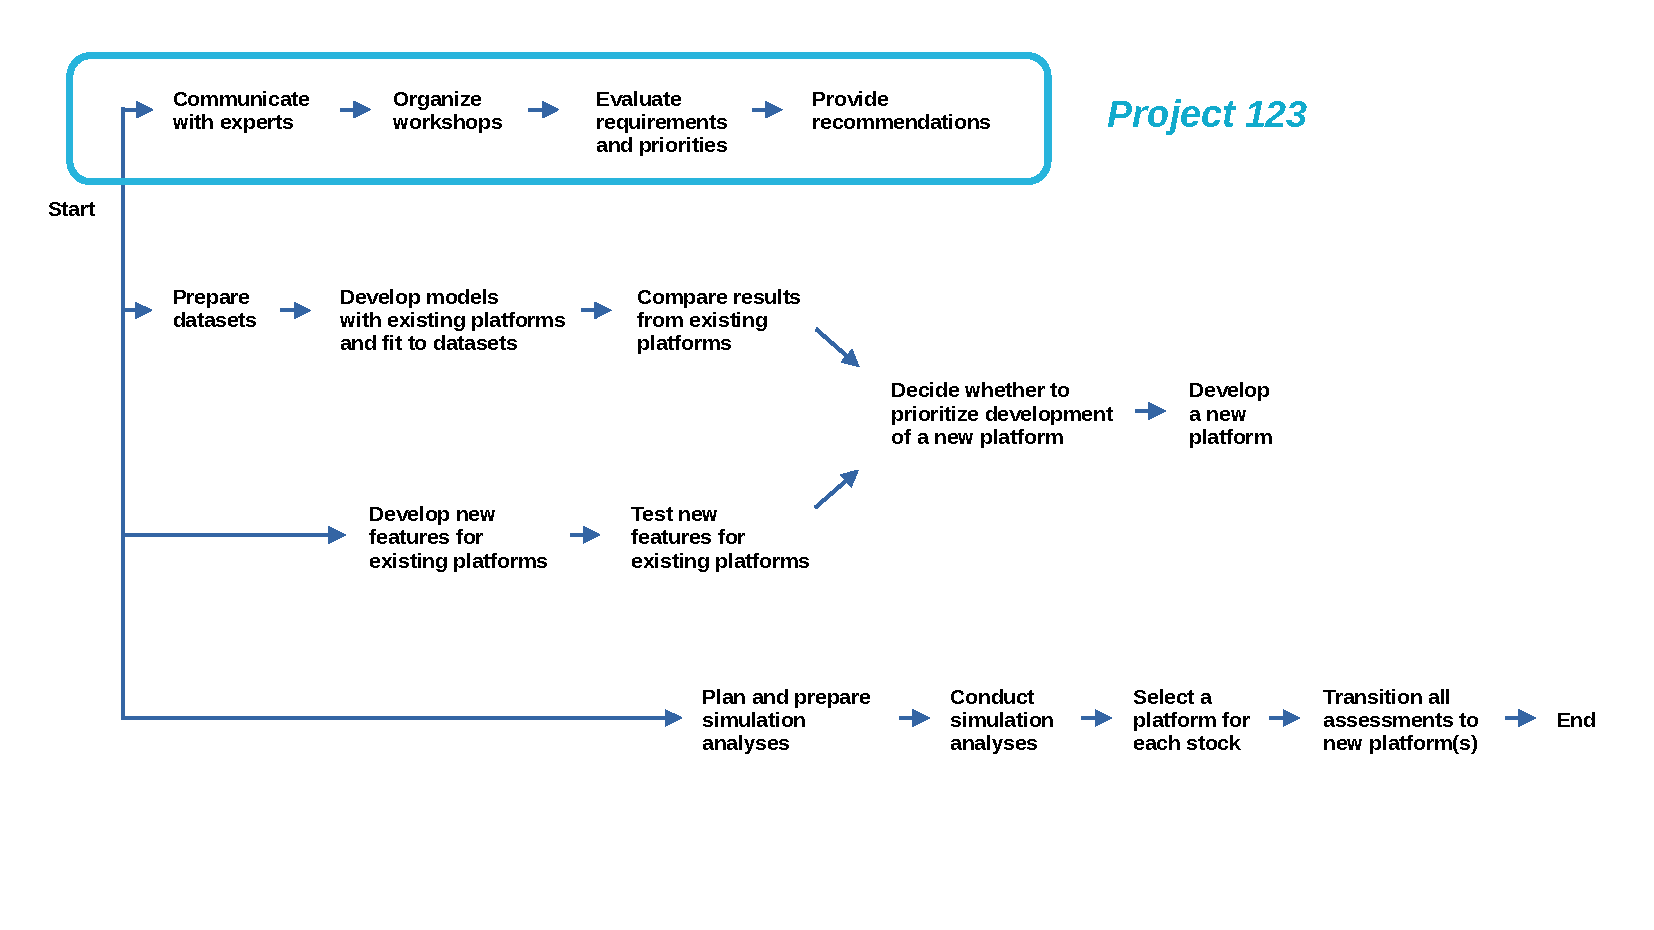
\includegraphics[width=0.95\paperwidth]{tasks}};
  \end{tikzpicture}
\end{frame}

% ______________________________________________________________________________

\begin{frame}{Meeting Schedule}\small
  \begin{tabular}{ll}
    \h{3ex}\gray 0:00\h{0.2ex}--\h{0.3ex}0:20
    & Introduction\\[1.6ex]
    \h{3ex}\gray 0:20\h{0.2ex}--\h{0.3ex}0:30
    & {\bf Platforms} currently used in tuna stock assessments
      {\gray (presentation, round table)}\\[1.6ex]
    \h{3ex}\gray 0:30\h{0.2ex}--\h{0.3ex}0:50
    & {\bf\green Common challenges} for all tuna RFMOs, {\bf\green longevity} of
      Stock Synthesis\\[0.6ex]
    ~ & and MULTIFAN-CL, {\bf\green succession plans} {\gray (round
        table)}\\[1.6ex]
    \h{3ex}\gray 0:50\h{0.2ex}--\h{0.3ex}1:00
    & SPC challenges and {\bf project plan} {\gray (presentation)}\\[1.6ex]
    $\Rightarrow$ \gray 1:00\h{0.2ex}--\h{0.3ex}1:10
    & {\bf Features} of current and future platforms {\gray
      (presentation)}\\[1.6ex]
    \h{3ex}\gray 1:10\h{0.2ex}--\h{0.3ex}1:25
    & Discussion on platform {\bf\green features} most {\bf\green relevant for
      tuna} {\gray (round table)}\\[1.6ex]
    \h{3ex}\gray 1:25\h{0.2ex}--\h{0.3ex}1:35
    & {\bf State-space} models and latest developments {\gray
      (presentation)}\\[1.6ex]
    \h{3ex}\gray 1:35\h{0.2ex}--\h{0.3ex}1:50
    & What do you think is the {\bf\green best way forward for SPC?} {\gray
      (round table)}\\[1.6ex]
    \h{3ex}\gray 1:50\h{0.2ex}--\h{0.3ex}2:00
    & Summary of discussions, next steps, {\bf collaboration} {\gray (round
      table)}\\[1.6ex]
  \end{tabular}
\end{frame}

% ______________________________________________________________________________

\begin{frame}{Features of Current and Future Platforms}\small
  \vspace{-1.5ex}
  \begin{columns}[T]
    \column{0.5\textwidth}
    \gray Incorporating data\\[-0.5ex]
    \begin{itemize}\fns
      \item Fit to length comps\\[-1ex]
      \item Fit to weight comps\\[-1ex]
      \item Fit to tagging data\\[-1ex]
      \item Fit to CKMR data\\[-1ex]
      \item Estimate growth curve using otolith data\\[-1ex]
      \item Utilize tag-recapture growth increment to estimate growth\\[3ex]
    \end{itemize}
    Specifics\\[-0.5ex]
    \begin{itemize}\fns
      \item Age-specific M\\[-1ex]
      \item Length-specific selectivity\\[-1ex]
      \item Region-specific growth
    \end{itemize}
    \column{0.5\textwidth}
    \gray Dimensions\\[-0.5ex]
    \begin{itemize}\fns
      \item Explicit regions with movement\\[-1ex]
      \item Tracking age and length in population\\[-1ex]
      \item Time steps within a year\\[3ex]
    \end{itemize}
    Ecology\\[-0.5ex]
    \begin{itemize}\fns
      \item Multispecies interactions\\[-1ex]
      \item Climate change\\[3ex]
    \end{itemize}
    Implementation\\[-0.5ex]
    \begin{itemize}\fns
      \item Random effects, state space\\[-1ex]
      \item Parallel computing\\[-1ex]
      \item Computation time
    \end{itemize}
  \end{columns}
\end{frame}

% ______________________________________________________________________________

\begin{frame}{Terms of Reference}\small
  \textit{2024}
  \begin{itemize}
    \item[1.] Review and identify important model features for tuna
    assessments\\[-1ex]
    \item[2.] Identify existing platforms that have these features or can be
    extended\\[-1ex]
    \item[3.] Reach out to and initiate collaboration with model
    developers\\[-1ex]
    \item[4.] Conduct two workshops in 2024, one online and one in person\\[4ex]
  \end{itemize}
  \textit{2025--2026}
  \begin{itemize}
    \item[5.] Explore and compare existing platforms, fitting to SPC tuna
    data\\[-1ex]
    \item[6.] Determine which platforms can be considered viable
    candidates\\[-1ex]
    \item[7.] If a viable platform has been identified, plan transition\\[-1ex]
    \item[8.] If no viable platform is identified, extend a platform or create a
    new one
  \end{itemize}
\end{frame}

% ______________________________________________________________________________

\begin{frame}{Software Platforms}\small
  Existing platforms that fit to length composition data
  \begin{itemize}
    \item[] Stock Synthesis\\[-1ex]
    \item[] Casal2\\[-1ex]
    \item[] Gadget\\[5ex]
  \end{itemize}
  Ongoing development
  \begin{itemize}
    \item[] SAM fitted to length comps \h{2.5ex}\comment{\fns Colin Millar,
      Anders Nielsen}\\[-1ex]
    \item[] WHAM fitted to length comps \comment{\fns Giancarlo Correa, Tim
      Miller}\\[-1ex]
    \item[] ALSCL \h{0.5ex}\comment{\fns Fan Zhang, Noel Cadigan}\\[-1ex]
    \item[] CCSBT \comment{\fns D'Arcy Webber, Rich Hillary}\\[-1ex]
    \item[] FIMS \h{2ex}\comment{\fns NOAA}\\[-1ex]
    \item[] SStag \h{2ex}\comment{\fns Nicholas Ducharme-Barth, Arni Magnusson}\\
  \end{itemize}
\end{frame}

% ______________________________________________________________________________

\begin{frame}{CAPAM 2019 Discussions}\small
  Tunas every 3 years\\[0.5ex]
  Swordfish every 4 years\\[0.5ex]
  Striped marlin every 5 years\\[2ex]
  \begin{itemize}
    \item[] {\bf 2024} ALB MLS\\[-1ex]
    \item[] {\bf 2025} SKJ SWO\\[-1ex]
    \item[] {\bf 2026} BET YFT\\[-1ex]
    \item[] {\bf 2027} ALB\\[-1ex]
    \item[] {\bf 2028} SKJ\\[-1ex]
    \item[] {\bf 2029} BET YFT SWO MLS\\[-1ex]
    \item[] {\bf 2030} ALB
  \end{itemize}
\end{frame}

% ______________________________________________________________________________


% ______________________________________________________________________________

\begin{frame}{Possible Outcomes}\small
  If commitment and funding is limited, then the following unwanted outcome,\\
  characterized by a lack of progress, could well occur...\\[2ex]
  \textit{Upcoming assessments:}
  \begin{itemize}
    \item[] {\bf 2024} MFCL with config changes, other platform(s) did not work
    well, workshop
    \item[] {\bf 2025} MFCL with config changes, other platform(s) did not work
    well, workshop
    \item[] {\bf 2026} MFCL without config changes, other platform(s) did not
    work well, workshop
    \item[] {\bf 2027} MFCL without config changes, other platform(s) did not
    work well, workshop
    \item[] {\bf 2028} MFCL without config changes, other platform(s) did not
    work well, workshop
    \item[] {\bf 2029} MFCL without config changes, other platform(s) did not
    work well, workshop
    \item[] {\bf 2030} MFCL without config changes, other platform(s) did not
    work well, workshop
  \end{itemize}
\end{frame}

% ______________________________________________________________________________

\begin{frame}{Possible Outcomes}\small
  will depend on:\\[3ex]
  \textbf{Level of funding}
  \begin{itemize}
    \item[] \textgreen{Level 0} ~--~ Annual workshops, coordination\\[-1ex]
    \item[] \textgreen{Level 1} ~--~ Hire one person for 5 years\\[-1ex]
    \item[] \textgreen{Level 2} ~--~ Hire two people for 5 years\\[5ex]
  \end{itemize}
  \textbf{Partnerships}
  \begin{itemize}
    \item[] Tuna RFMOs ~--~ funding and scientists' time\\[-1ex]
    \item[] Domain experts in state-space model development ~--~ scientists'
    time\\[-1ex]
    \item[] Other funding sources\\[1ex]
  \end{itemize}
\end{frame}

% ______________________________________________________________________________

\begin{frame}{Summary}
  \begin{itemize}
    \item[] {\bf\darkblue Project P123} \comment{objective, background,
      terms of reference}\\[5ex]
    \item[] {\bf\darkblue Software Platforms} \comment{operational, current and
      future development}\\[5ex]
    \item[] {\bf\darkblue Road Ahead} \comment{assessments, workshops,
      collaboration, adaptive plan}\\[5ex]
    \item[] {\bf\darkblue Possible Outcomes} \comment{level of funding,
      partnerships}\\[1ex]
  \end{itemize}
\end{frame}

\end{document}
